\subsection{Theoretical Motivation}
\label{sec:theory}

Two propositions underpin the scheduler design.
At timestep~$t$, given the current latent~$x_t$, each noise candidate
$\varepsilon_t\sim\mathcal{N}(0,I)$ induces a verifier score through the
chain defined in \cref{eq:x0_prediction,eq:score}:
\begin{equation}
  S_t \;=\; v\!\bigl(\,D_\theta\bigl(F_\theta(x_t,\,t,\,c,\,\varepsilon_t),
  \;t\!-\!1,\;c\bigr),\;c\bigr).
  \label{eq:score_rv}
\end{equation}
Since the only randomness is in~$\varepsilon_t$, $S_t$ is a random variable
whose distribution we denote $\mathcal{D}_t(c,x_t)$; it depends on the
prompt~$c$ and the current latent~$x_t$ (itself a function of all prior
noise choices).
Write $\mu_t=\mathbb{E}[S_t]$ and $\sigma_t^2=\operatorname{Var}(S_t)$.
Local search with $K$ candidates returns the maximum order statistic
$M_t^{(K)}=\max_{k\le K}S_t^{(k)}$, whose expected gain over a single draw
is
\begin{equation}
  G_t(K) \;=\; \mathbb{E}\!\bigl[M_t^{(K)}\bigr] - \mu_t.
  \label{eq:gain}
\end{equation}
When the score distributions $\{\mathcal{D}_t\}$ form a
\emph{location-scale family}---i.e.,
$S_t = \mu_t + \sigma_t Z$ for a common standardized variable $Z$
whose distribution does not depend on~$t$---the gain factorizes as
\begin{equation}
  G_t(K) \;=\; \sigma_t\,a_K,
  \qquad
  a_K \;\triangleq\; \mathbb{E}\bigl[\max(Z_1,\dots,Z_K)\bigr],
  \label{eq:gain-factor}
\end{equation}
where $Z_1,\dots,Z_K\stackrel{\text{iid}}{\sim}Z$.
The sequence $a_K$ is universal (independent of~$t$) and depends only
on the shape of~$Z$.
For the Gaussian case $Z\sim\mathcal{N}(0,1)$, $a_K$ coincides with
the expected maximum of $K$ standard normals (David and Nagaraja, 2003,
Ch.~4); but the factorization holds equally for any location-scale
family (e.g., logistic, Laplace).
Since $a_K$ is concave and increasing in $K$ with $a_1=0$, the gain function
$G_t(K)$ inherits concavity: additional candidates yield diminishing
returns, with the rate of diminishment governed by~$\sigma_t$.

The global scheduling problem is to allocate the total budget $B$ across
timesteps to maximize the aggregate gain:
\begin{equation}
  \max_{K_1,\dots,K_T}\;\sum_{t=1}^{T}G_t(K_t)
  \quad\text{s.t.}\;\sum_{t=1}^{T}K_t=B,\;K_t\ge 1.
  \label{eq:alloc}
\end{equation}

\begin{proposition}[Offline profiling under independence]
\label{prop:offline}
Suppose $\mathcal{D}_t(c,x_t)=\mathcal{D}_t$ for all $c,x_t$ (prompt-
and history-independent scores).
Then:
\begin{enumerate}
\item[\textbf{(i)}]
  Problem~\eqref{eq:alloc} decomposes across timesteps: any optimal
  allocation $\{K_t^*\}$ is simultaneously optimal for every prompt.
\item[\textbf{(ii)}]
  The optimal allocation equalizes marginal gains:
  $G_t'(K_t^*)=\lambda^*$ for all~$t$ with $K_t^*>1$,
  where $\lambda^*$ is the Lagrange multiplier on the budget constraint.
  Under any location-scale family, $K_t^*$ is increasing in~$\sigma_t$.
\item[\textbf{(iii)}]
  $\sum_t G_t(K_t^*) > \sum_t G_t(B/T)$ whenever
  $\{\sigma_t\}$ are not all equal, and the gap grows with the
  dispersion of~$\{\sigma_t\}$.
\end{enumerate}
\end{proposition}

\cref{prop:offline} justifies the offline profiling stage.
Part~(i) shows that under the independence assumption, a single fixed
allocation is optimal for all prompts, so profiling on a small calibration
set generalizes.
Part~(ii) reveals a water-filling structure: timesteps with wider score
distributions---those where noise perturbations matter most---receive more
budget.
Part~(iii) quantifies the advantage of non-uniform allocation: the more
heterogeneous the per-step variances $\{\sigma_t\}$, the larger the gain
over uniform scheduling.

\begin{proposition}[Online adaptation under prompt dependence]
\label{prop:online}
Suppose $\mathcal{D}_t(c,x_t)$ varies with the prompt and search history
(location-scale case: $\sigma_t = \sigma_t(c,x_t)$).
Define the oracle value
$V^*(\boldsymbol{\sigma})=\max_{\{K_t\}:\sum_t K_t=B}\sum_t\sigma_t\,a_{K_t}$
for variance profile $\boldsymbol{\sigma}=(\sigma_1,\dots,\sigma_T)$.
Then:
\begin{enumerate}
\item[\textbf{(i)}]
  $V^*$ is convex in $\boldsymbol{\sigma}$.
  The expected regret of any fixed allocation satisfies
  \begin{equation}
    \mathbb{E}_{\boldsymbol{\sigma}}\!\bigl[V^*(\boldsymbol{\sigma})\bigr]
    \;-\; V^*\!\bigl(\bar{\boldsymbol{\sigma}}\bigr) \;\ge\; 0,
    \label{eq:jensen-gap}
  \end{equation}
  where $\bar{\boldsymbol{\sigma}}=\mathbb{E}[\boldsymbol{\sigma}]$,
  with equality iff $\boldsymbol{\sigma}$ is constant across instances.
\item[\textbf{(ii)}]
  Under any location-scale model, the marginal gain factorizes as
  \begin{equation}
    G_t'(K) \;=\; \underbrace{\sigma_t}_{\text{sensitivity}}
    \;\cdot\; \underbrace{a_K'}_{\text{exhaustion}}.
    \label{eq:marginal-decomp}
  \end{equation}
  The optimal stopping condition is $G_t'(K)\le\lambda^*$, the shadow
  price of budget.
  The running mean $\bar{g}$ satisfies
  $\bar{g}\ge\tfrac{1}{|\mathcal{H}_g|}\sum_s G_s'(\hat{K}_s)$
  by concavity, so $\beta_g\bar{g}$ estimates~$\lambda^*$.
  The gain condition $\widetilde{g}_t^{(j)}<\beta_g\bar{g}$ tests the
  product $\sigma_t\,a_K'\le\lambda^*$; the variance condition
  $\hat{\sigma}_t^{(j)}<\beta_\sigma\bar{\sigma}$ independently tests
  $\sigma_t\le\bar{\sigma}$.
  Requiring both conditions prevents premature stopping at
  high-value timesteps: under estimation noise, either threshold
  alone can be falsely triggered while the other factor remains
  large, so the conjunction avoids abandoning timesteps that still
  offer substantial search potential.
\end{enumerate}
\end{proposition}

\cref{prop:online} motivates the online controller.
Part~(i) shows that the oracle value $V^*$ is convex in the variance
profile---a pointwise maximum of linear functions---so by Jensen's
inequality, any fixed allocation based on the population mean
$\bar{\boldsymbol{\sigma}}$ leaves an expected gap
(\cref{eq:jensen-gap}) that grows with the cross-instance variability
of~$\boldsymbol{\sigma}$.
Part~(ii) reveals that the marginal gain~\eqref{eq:marginal-decomp}
is a product of two independent factors, each monitored by a separate
threshold.
Low gain with high variance ($a_K'$ small, $\sigma_t$ large) means
the current timestep is responsive but exhausted at this iteration
count---yet a lucky draw may still yield a large jump, so stopping is
premature.
Moderate gain with low variance ($a_K'$ moderate, $\sigma_t$ small)
means the timestep is inherently insensitive and gains will plateau
regardless---but at this moment the search is still productive.
Only when \emph{both} factors are small is stopping unambiguously
justified.
\cref{fig:stopping} illustrates this two-threshold logic.

\begin{figure}[t]
\centering
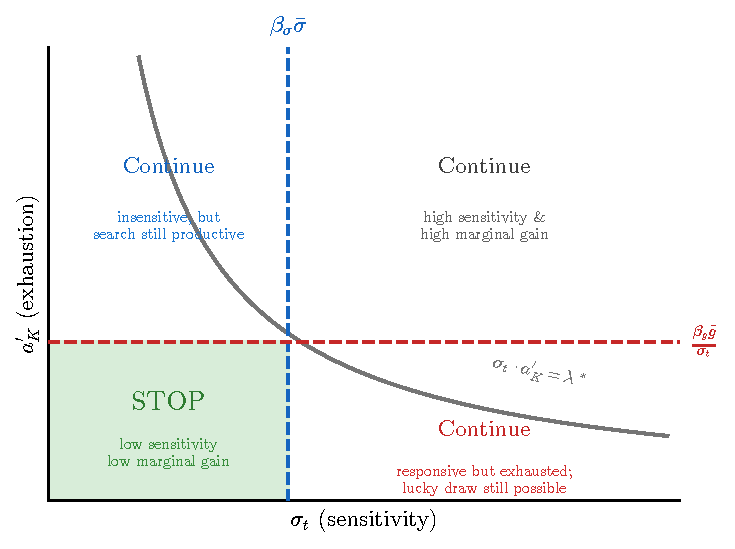
\includegraphics[width=0.75\linewidth]{figures/fig_stopping_decision.pdf}
\caption{Online stopping decision in the $(\sigma_t, a_K')$ plane.
The variance threshold (vertical dashed) and gain threshold (horizontal dashed)
partition the space into four regions.
Stopping is triggered only when \emph{both} conditions are met (shaded region),
corresponding to the conjunction in \cref{prop:online}(ii).
The hyperbola $\sigma_t\cdot a_K'=\lambda^*$ shows the true optimality boundary;
the rectangular approximation is conservative by design.}
\label{fig:stopping}
\end{figure}

Proofs are given in \cref{sec:proofs}.
